\section{Introduction} \label{intro}
\subsection{The Definition} \label{def}

The aim of this paper is to eventually define the Lebesgue Intergral - so lets just try to do that straight away.
\begin{definition}
	Given
	\begin{itemize}
		\item a Measure Space; $(X, \A, \mu)$,
		\item an $\A/\eB$ Measuarable Function $u : X \rightarrow \eR$,
		\item positive functions $u^+$ and $u^-$ s.t. $u = u^+ - u^-$,
		\item the sets $S^{\pm}$ of {\em all} Simple Functions ($S \subset \E_\mu^+$) on $(X, \A, \mu)$ s.t. $s \in S^{\pm} \Rightarrow s \leq u^{\pm}$,
	\end{itemize}

	we define the $\mu$-integral of u - which we write as $\int u\,d(\mu)$ - in terms of the integrals of the positive functions $u^+$ and 			$u^-$. The intergral of a general positive function - so including our $u^{\pm}$ - is defined as

	\begin{equation*}\label{posint}\tag{\ref{L}$'$}
	\int u^+\,d(\mu) \coloneqq \sup\bigr\{ I_\mu(s) : \ \  s \in \E^+ \hbox{ \ and \ } s \le u \bigl\},
	\end{equation*}

	and going back to our more general u, 

	\begin{equation}\label{L}
	\int u\,d(\mu) \coloneqq \int u^+\,d(\mu) - \int u^-\,d(\mu).
	\end{equation}

	If the domain of our function is $\R^n$, with the 'standard' $n$-dimensional Borel $\sigma$-algebra and Lebesgue Measure on it - i.e. $(X, \A, \mu) 	= (\R, \B, \lambda^n)$ - then this becomes the $\lambda^n$-integral (read as Lebesgue integral instead of lambda integral - or we just 			call it 'the integral') and we write

	\begin{equation*} \tag{\ref{L}$''$}
	\int u\,d(\lambda^n) =  \int u(x)\,d(\Ln) \coloneqq \int u(x)\,d(x) 
	\end{equation*}
\end{definition}

That's quite a long definition, one which raises more questions than it answers. The first (and biggest) issue here is that, even assuming someone has taken a course in Analysis, there are many undefined terms;
\begin{itemize}
	\item What are Measures and $\sigma$-algebras? And what is a Measure Space?
	\item What is the Borel $\sigma$-algerbra
	\item What is a Measuarable Function? What is a Simple Function?
	\item What is $I_\mu$ and why can it seemingly only be used on positive Simple Functions?
\end{itemize}

That last bullet point touches on the second key issue with this definition; why. Why any of this. What about this definition of what we call the integral makes it any better than the Reimann Integral? Do they even describe similar things? This is not at all immedately obvious, since the Reimann intergral is defined on functions $f: Y \rightarrow \R$ where Y is some compact\footnote{Define a compact set} subest of R and this integral is defined on...well, any set at all.

Even if we can somehow convince ourselves they are compatible, it still seems like a convoluted defintion - what about Simple Functions is so special that the intergrals of all other functions are defined in terms of them (or to be more precise, why are general functions are defined in terms of positive functions, and then positive functions defined in terms of positive simple ones)?

Interestingly (to me, at least) the Reinmann intergral is defined in a similarish way - we find the upper Reimann intergral of a function by finding all the Step Functions which bound the function from above, define/find the intergrals of these using their 'steppyness', then take the infinium - we do the same thing from below, and then if these limits coiencied then we call that the Reinmann integral. In order to understand the motivations behind Lebegsue Intgration better, let's take a slightly closer look at the similarites and differences between these two.
\newpage
% !TeX root = Project.tex
\section{Riemann vs. Lebesgue}
%
%
\subsection{The Motivation}
Our goal when we integrate a function is to find the amount of `space' between the graph and x-axis (or the Abscissa if you're fancy). It's pretty difficult to say how much space an arbitrary curve takes up, but we can work out the area of rectangles very easily --- by calculating the {\em base $\times$ height}. Riemann integration takes advantage of this, and defines the integral of a function $f:\R \rightarrow \R$ by first bounding it from above with rectangular functions and finding the smallest of these areas (which is would be an upper bound for the area of the function), then we bound the function from below and find an lower bound, then we hope that these two bounds match up. 

\begin{figure}[H] % Remember to change this to 'h'!
	\renewcommand{\subfigcapskip}{-5pt}
	\centering
	\subfigure[Bounding from Below.]{%
		\label{fig:areabelow}
		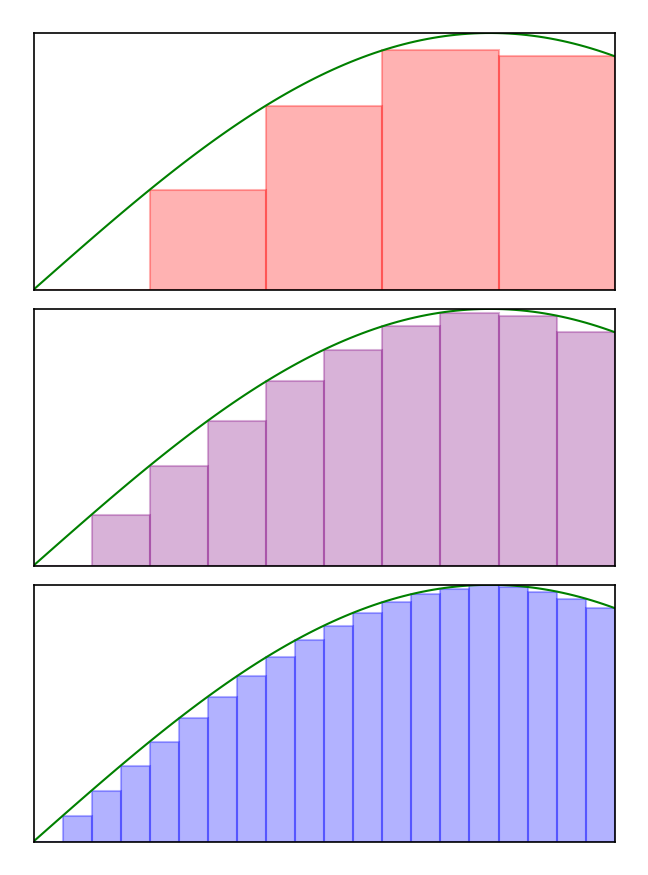
\includegraphics{Code/Area3.png}}
	\subfigure[Bounding from Above.]{%
		\label{fig:areaabove}
		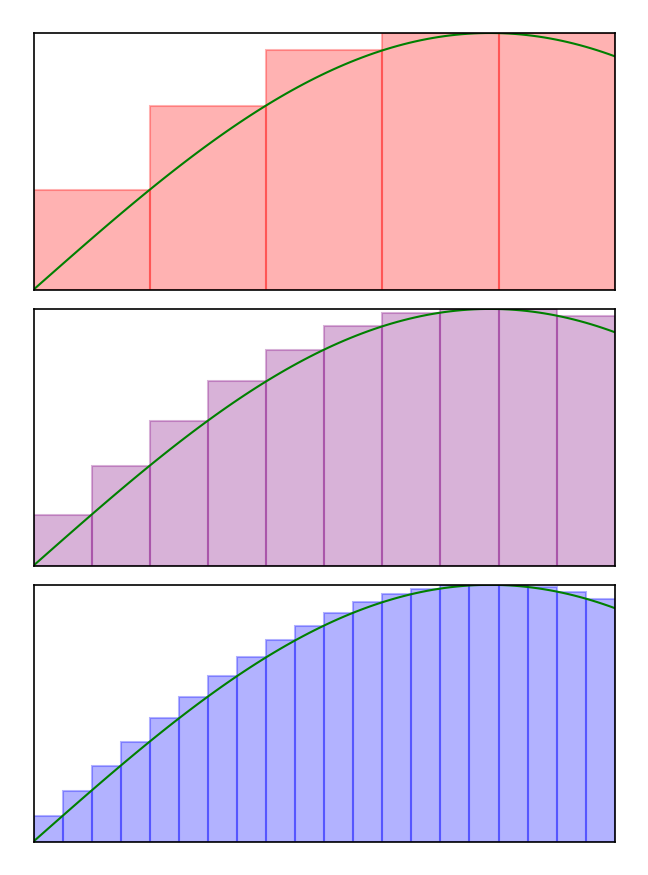
\includegraphics{Code/Area4.png}}
	\caption{Approximating Area with Step Functions.}
	\label{fig:areaapprox}
\end{figure}

If the domain of our function (the `x-axis'), is $\R^2$ instead of just $\R$, we'd actually calculating a volume by finding the `space' between the graph and the axis. Curves are bad enough, but it's even harder to find the volume under a surface. Basic Riemann Integration doesn't apply to these functions --- but if we wanted, we could make a similar observation and simpification. The analog to a rectangle in $\R^3$ is a cuboid, and we and think of its size as being calculated in much the same way as in $\R^2$; the size of the base (which is now an area, instead of a length) $\times$ the height. It'd be nice if there were a way to take advantage of this so that we could integrate any function where we can make sense of \emph{`the size of the base.'} With this is mind, lets clear up some of the terms we are going to use:

\begin{description}
\item[\em Lebesgue integration\/] is the method of integration defined above. Just like Riemann Integration, it is used to find the space between the graph of a function and the domain. However, unlike Riemann, the domain can be any set at all. Thinking back to rectangles and cuboids and $base \times height$, if we wanted make sense of what it means for there to be space between the graph and the x-axis, we should be able to make sense of the `size' of parts of the domain, so that we can figure out how big our base is and multiply that by the height$\ldots$
%
\item[\em The Lebesgue Measure\/] seems then like it'd be a way to assign sizes to, or `measure' sets any domain; but it is not! It's a term used specifically when we give sizes to the subsets of $\R^n$, and those sizes (or `measures') coincided with our usual idea of the size of a set in $\R^n$ --- i.e. it is used when we are considering functions $\R^n \supset Y \rightarrow \R$, and in $\R$ the measure (length) of the interval $[1, 0]$ is 1, in $\R^2$ the measure (area) of the rectangle $[1, 0] \times [1, 0]$ is 1, in $\R^3$ the measure (volume) of the cube $[1, 0] \times [1, 0] \times [1, 0]$ is 1$\ldots$ etc. 
%
\item[\bf \em The Lebesgue Integral\/] is what we get when we do Lebesgue Integration on a set with the Lebesgue Measure on it. i.e. it's Integral of normal functions $\R^n \supset Y \rightarrow \R$. This is the (basically) the same domain as the Riemann integral and so we'd want to check that the Lebesgue Integral and the Riemann integral match up --- and then see if the Lebesgue integral is better in some way.
\end{description}

Already, we can see an improvement over Riemann Integration; \emph{Lebesgue Integration} is defined on any set at all (kind of), and even the more restricted \emph{Lebesgue Integral} can be calculated directly for any $\R^n$ --- so no double/triple integration nonsense. To see another benefit of the Lebesgue Integral over Riemann, let's look at the canonical example of a function for which the Riemann Integral fails; $f\colon \R \rightarrow \R,\ \ f(x) = \mathbbm{1}_\Q(x)$ (Figure \ref{fig:rational}). This is also an example of a \emph{Simple Function} since it is just the \emph{Indicator Function} of a measurable set, but lets not get ahead of ourselves$\ldots$ First, we should define the Riemann Integral. 

% !TeX root = Project.tex
\subsection{The Definition of the Riemann Integral}
The definition of the Riemann Integral involves a few steps, and so it's going to take a little patience. The first step is defining a \dref{def:stfun}[\emph{Step Function}] - no pun intended.
%
\begin{figure}[h]
	\centering
	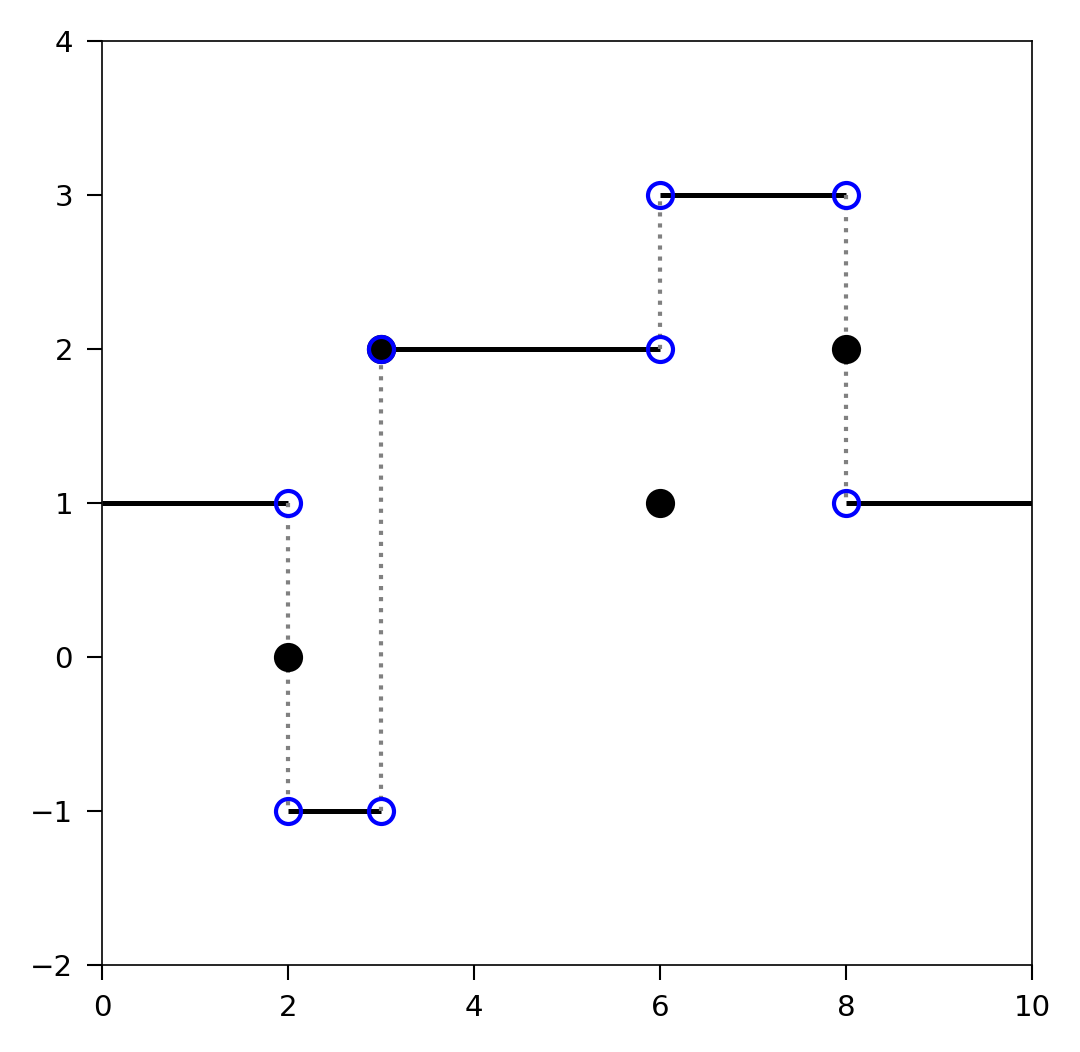
\includegraphics{Code/Step.png}
	\caption{A Step Function}
	\label{fig:step}
\end{figure}

A function is called a \dref{def:stfun}[\emph{Step Function}] if and only if there exists some finite sequence of points such that the function is constant between any two adjacent points. So, for the function with the graph shown in Figure \ref{fig:step}, the points $\{0, 2, 3, 6, 8, 10\}$ are a finite sequence which make this a step function. We will often index the elements of sequence using $n$, and label each element $x_n$. We can call sequence this a \emph{`representation'} of the function, and we can call the sequence of constant heights taken just \emph{before} the $n^{th}$ point in our representation the corresponding \emph{`height sequence'}. The \emph{\label{def:hseq}{\color{Magenta}height sequence}} along with the representation fully describe the function.

\medskip
Note two important points;
\begin{itemize}
	\item We could have picked $\{0, 1, 2, 3, 4, 5, 6, 7, 8, 9, 10\}$ to be our representation, since the function also happens to constant between any two adjacent integers. 
	\item It doesn't really matter what the function is {\em at} the points $x_n$ --- we only care whether the function is constant {\em between} our given points. In our graph, 2, 3, 6, and 8 are discontinues, but that doesn't matter since they're also in our sequence of points. 
\end{itemize}

The formal definition is as follows;
\begin{definition}[Step Function]\label{def:stfun}
Given $\phi\colon \ [a, b] \rightarrow \R$, $\phi$ is a {\color{Magenta}\emph{Step Function}}
    \begin{itemize}
        \item[$\logeq$]
            $\phi \in {\color{Magenta}\mathcal{S}([a, b])}$
        \item[$\logeq$]
            $\exists N \! \in \! \N$ \ : \ $\exists {\color{Magenta}X} = (x_n)_{n=0}^N$ : $a = x_0 < x_1 < \ldots < x_{n-1} < x_n = b$, \ and \ $\forall m\in\N_{< N}$ we have $\exists! c_m \in \R$ : $\forall z \in (x_{m-1}, x_{m})$ we have $\phi(z) = c_m$.
    \end{itemize}
\end{definition}

This also defines \emph{the set of all step functions on} $[a, b]$ as \dref{def:stfun}[\emph{$\mathcal{S}[a, b]$}]. This kind of thing is done a lot in analysis --- we often want to look at the set of all things which satisfy some property. We normally don't have to \emph{find} them all --- we just need a way to represent the full set. The fact that it'd be near impossible to try to imagine the set \dref{def:stfun}[\emph{$\mathcal{S}[a, b]$}] is irrelevant --- it's just important we know it exists. The sequence \dref{def:stfun}[$X$] is a representation.

\medskip
Next, we want to define what it means to \dref{def:stint}[\emph{Integrate}] a step function. Remember, the point of working with step functions is because it's easy to find the area of rectangles, and integration is all about finding areas. So where are the rectangles? 

\medskip
As is hinted at by Figure \ref{fig:step}, we can make the bases of the rectangles the widths of the intervals $(x_{n-1}, x_n)$, and the heights the constant $c_n$s which values in these interval take. This is made even clearer by Figure \ref{fig:stepfilled}, where we can also see that the sometimes our heights will have negative values, and that's okay --- these areas are just taken away from the total area instead of added.
 
 \medskip
What's not okay is that any one step function may have different sequences which we can use to prove that it's a step function --- or in other words, the same step function may have different but equally valid representations. We want to define the integral of a step function in terms it's representation, but how do we know that different representations of the same function produce the same integral? Figure \ref{fig:stepfilled} demonstrates that, given the representations $\{0, 2, 3, 6, 8, 10\}$ and $\{0, 1, 2, \ldots, 10\}$ of \ref{fig:step}, we're fine, and the areas are equal. \tref{thm:repuni}[It turns out] that this is the case in general --- the integral of a step function is independent of the chosen representation.

\begin{figure}[h]
  \centering
  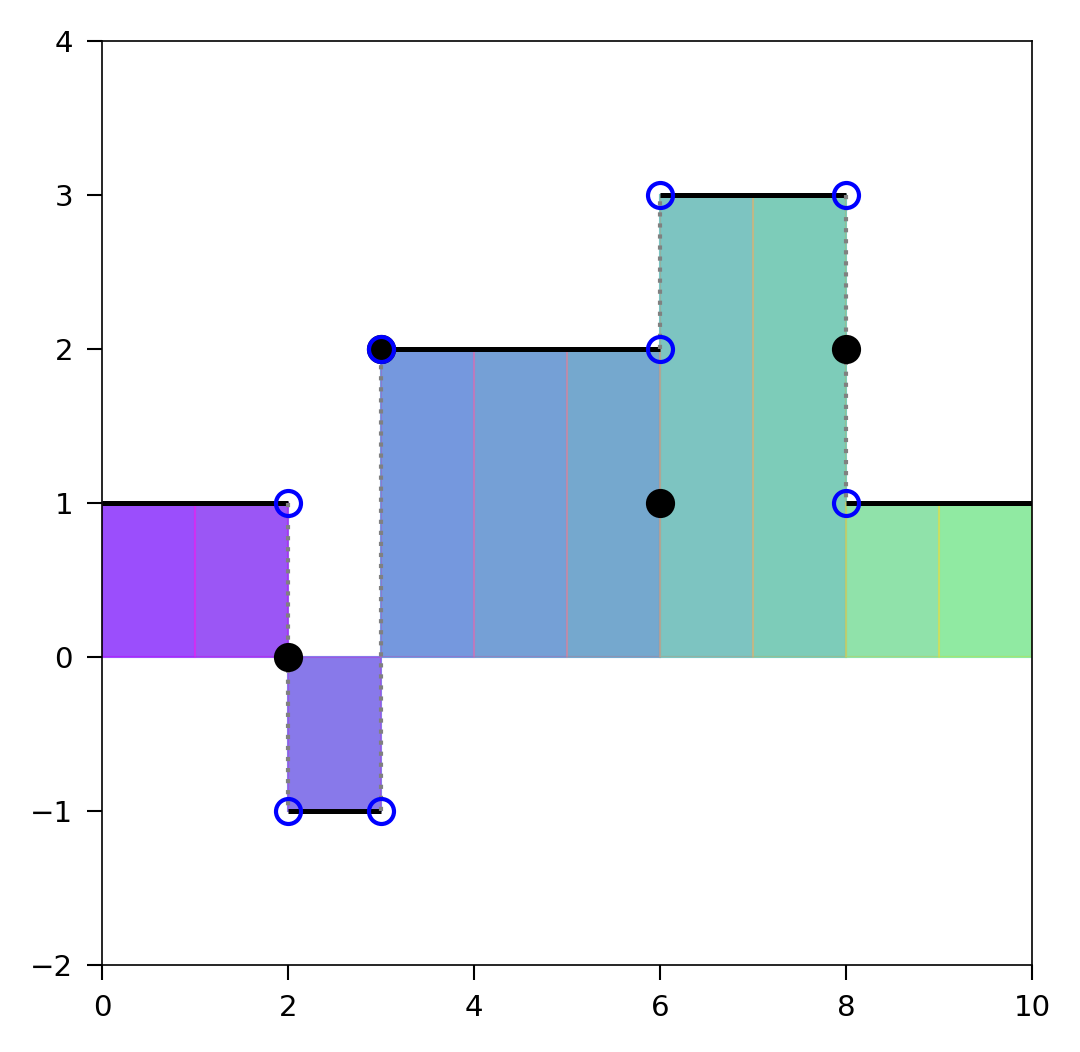
\includegraphics{Code/StepFilled2.png}
  \captionof{figure}{Integral of \ref{fig:step}}
  \label{fig:stepfilled}
\end{figure}

\begin{definition}[Integral of a Step Function]\label{def:stint}
	Given
	\begin{itemize}
	\item 
		$\phi \in \mathcal{S}([a, b])$,
	\item
		$N \in \N$ and the representation $(x_n)_{n=0}^N$ of $\phi$,
	\item
		the corresponding \emph{height sequence} $(c_n)_{n=1}^N : \phi(x) = c_n \quad \forall x \in (x_{n-1}, x_{n})$,
	\end{itemize}
	then the {\color{Magenta}\emph{Integral}} of $\phi$ as a function of $x$ on $[a, b]$ is
	\begin{equation}
	\begin{split}
		&{\color{Magenta}\intx{\phi(x)}} \\
		\defeq \quad &\sum_{i=1}^N c_i(x_{i} - x_{i-1}).
	\end{split}
	\end{equation}
\end{definition}%

To show that the Integral is independent of the choice of representation, we'd need to show that if we had two arbitrary representations $(x_n)_{n=0}^N$ and $(x'_m)_{m=0}^M$ with \emph{height sequences} $(c_n)_{n=1}^N$ and $(c'_m)_{m=1}^M$ resp. then, $$\sum_{i=1}^N c_i(x_{i} - x_{i-1}) = \sum_{j=1}^M c'_j(x'_{j} - x'_{j-1}).$$ 
The idea behind why this is true is the following; 
\begin{itemize}
\renewcommand\labelitemi{$\times$}
\item
Assuming first that one sequence is a subsequence of the other, we will focus on the representation that is more `fine' --- i.e. the one that has smaller width rectangles; ones which are divisions of the rectangles in the `coarser' representation. 
\item
We look at it in sections; with the sections being the steps of the coarser representation. So, in \ref{fig:step}, we'd look at $\{0, 1, 2 \ldots, 10\}$ between 0 and 2, then 2 and 3, then 3 and 6 $\ldots$ etc. 
\item
The two representations are for a single the step function; and we use this group adjacent rectangles with the same height. $\phi(x)$ must be constant in the section we are looking at, and so we know that all the rectangles here have the same height
\item
Then we can use the distributive property of multiplication to view the smaller width rectangles of the same height as one big rectangle with the width of the whole section. And boom, we're done, since those big rectangles are exactly the ones which you would use when integrating using the coarser representation.
\item[$\otimes$]
If neither representation is contained within the other, then we can just create a third representation which is the union the first ones. Both original sequences will be coarser than this new one, and so we can use the same reasoning as before, plus transitivity and symmetry, to prove the integrals are the same.
\end{itemize}

\begin{figure}[h]
	\renewcommand{\subfigcapskip}{-5pt}
	\centering
	\subfigure[Focus on finer representation.]{%
		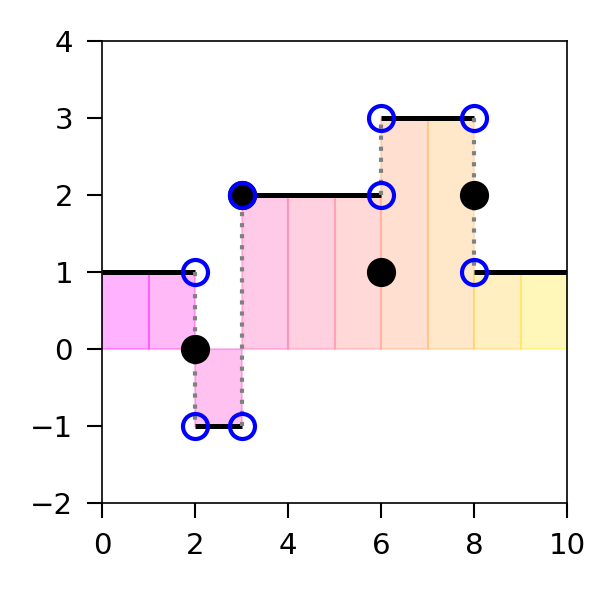
\includegraphics{Code/StepFilledSmall.png}}\qquad
	\subfigure[Look at section between 3 and 6.]{%
		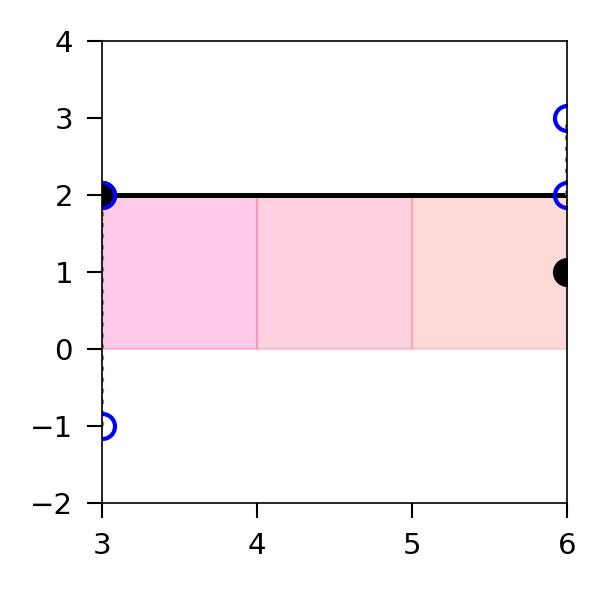
\includegraphics{Code/StepFilledFocused.png}}\\
	\subfigure[Group rectangles.]{%
		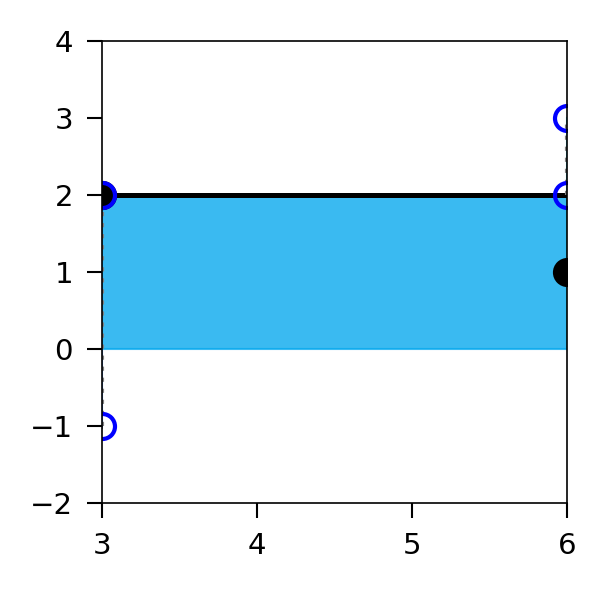
\includegraphics{Code/StepFilledFocused3.png}}\qquad
	\subfigure[\bf Boom]{%
		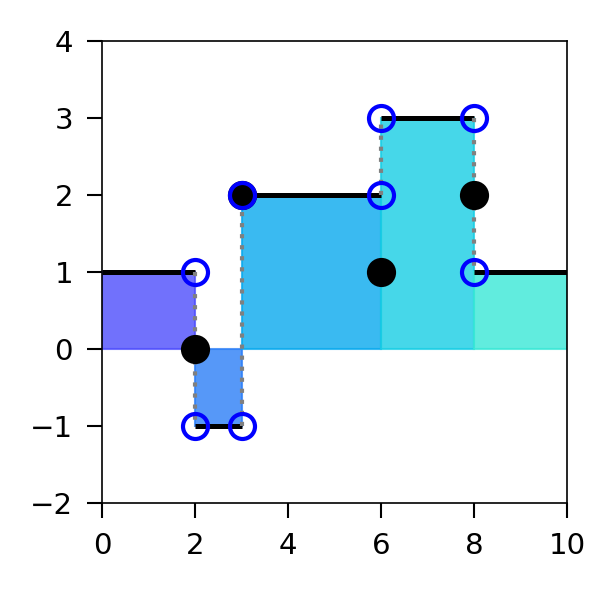
\includegraphics{Code/StepFilled3Small.png}}
	\caption{Different representations of the same function.}
	\label{fig:representations}
\end{figure}

\begin{prop}\label{thm:repuni}
	Given,
	\begin{itemize}
		\item
		$\phi \in \allstep$,
		\item
		$N, M [=N'] \in \N$ and the representations $(x_n)_{n=0}^N$ and $(x'_{m [=n']})_{m=0}^M$ of $\phi$,
		\item
		The respective height sequences $(c_n)_{n=1}^N$ and $(c'_m)_{m=1}^M$ of these representations,
	\end{itemize}
	then
	\begin{equation}
	\sum_{i=1}^N c_i(x_{i} - x_{i-1}) = \sum_{j=1}^M c'_j(x'_{j} - x'_{j-1}).
	\end{equation}
\end{prop}
\begin{cproof} 
	\leavevmode \\
	\emph{Case 1:} $\{x_n; n \in \N_{n<N}\} \subset \{x'_m; m \in \N_{m<M}\}$:
	\begin{IEEEeqnarray}{rCl}
		&  & \{x_n; n \in \N_{<N}\} \subset \{x'_m; m \in \N_{<M}\} \nonumber \\
		& \Leftrightarrow \quad & \exists J = (j_n)_{n=0}^N \nonumber \\
		&  & : 0 = j_0 < j_1 < \ldots < j_{n-1} < j_n = m \text{ and } k \in \N_{<N} \text{ we have } x_k = x'_{j_k} \nonumber
	\end{IEEEeqnarray}
	Hence,
	\begin{IEEEeqnarray}{rCl}
	\sum_{j=1}^M  c'_j(x'_{j} - x'_{j-1})  & = & \sum_{k=0}^N \; \sum_{j = j_{k-1}}^{j_k} \!\! c'_j(x'_{j} - x'_{j-1}) \nonumber \\
	& = & \sum_{k=0}^N \; c'_{j_k} \!\!\! \sum_{j = j_{k-1}}^{j_k} \!\! (x'_{j} - x'_{j-1}) \nonumber \\
	& = & \sum_{k=1}^N  c_k(x_{k} - x_{k-1}) \nonumber 
	\end{IEEEeqnarray}
	\emph{Case 2:} Arbitrary representations $X = \{x_n; n \in \N_{<N}\} \text{ and } X' = \{x'_{n'}; n' \in \N_{<N'}\}$:

	\medskip
	Let $X'' = \{x''_{n''}; x"_{n''} \in X\cup X'\}$.
	\begin{IEEEeqnarray}{rCc}
		&  & \{x_n; n \in \N_{n<N}\} \subset \{x''_{n''}; n'' \in \N_{<N''}\} \supset \{x'_{n'}; n' \in \N_{m<M}\} \vspace{3pt}\nonumber \\
		& \Rightarrow \quad & \sum_{X} = \sum_{X''} = \sum_{X'} \nonumber 
	\end{IEEEeqnarray}
\end{cproof}
%
%
%
Now we are ready to define the \dref{def:riemann}[\emph{Riemann Integral}] of any function $f\colon [a, b] \rightarrow \R$ $\ldots$ almost. We first need to define 2 separate upper and lower integrals, and then if they are the same, what we call that the \emph{Riemann Integral} of the function. This is actually why $\mathbbm{1}_\Q(x)$ is not \emph{Riemann Integrable}; it's upper and lower integrals do not coincide. 

\medskip
To find the \dref{eq:upperriemann}[\emph{Upper Riemann Integral}] of $f$, first find \emph{all} the step functions which bound it from above, then calculate their integrals using \drefn{def:stint} and then, finally, define the smallest of these integrals to be the Upper Riemann Integral. To find the \dref{eq:lowerriemann}[\emph{Lower Riemann Integral}], you do the same thing, but from below. The set of all Riemann Integrable functions on $[a,b]$ is \dref{eq:riemann}[\emph{$\mathcal{R}([a, b])$}].

\medskip
Figure \ref{fig:areaapprox} tries to illustrate this, but it's important to remember that we aren't looking at a sequence of step functions, we are looking at \emph{all of them}. How to calculate/approximate integrals using sequences of [step] functions is a whole thing in itself --- I wish I had started writing this sooner so that I could get into it because it's super interesting, but alas$\ldots$ Anyway, now we can define Riemann Integration for real:

\begin{definition}[Riemann Integration]\label{def:riemann}
	Given  
	\begin{itemize}
	\item
		$f\colon [a, b] \rightarrow \R$,
	\item
		$S_l \subset \allstep : \psi \in S_l \Leftrightarrow \ \psi(x) \leq f(x) \quad \forall x \in [a, b] $,
	\item
		$S_u \subset \allstep : \phi \in S_u \Leftrightarrow \ \phi(x) \geq f(x') \quad \forall x' \in [a, b] $,
	\end{itemize}
	then the {\color{Magenta}\emph{Lower Riemann Integral}} of $f$ is
	\begin{equation}
		{\color{Magenta}\underline {\int}} \, f(x) \, dx \defeq \sup \left\{\intx{\psi(x)}; \;\; \psi \in S_l\right\}
		\label{eq:lowerriemann}
	\end{equation} 
	and the {\color{Magenta}\emph{Upper Reimann Integral}} is
	\begin{equation}
		{\color{Magenta}\overline {\int}} \, f(x) \, dx \defeq \inf \left\{\intx{\phi(x)}; \;\; \phi \in S_u\right\}.
		\label{eq:upperriemann}
	\end{equation}
	If \eqref{eq:lowerriemann} = \eqref{eq:upperriemann}, then $f$ is {\color{Magenta}\emph{Riemann Integrable}} the {\color{Magenta}\emph{Riemann Integral}} of $f$ as a function of $x$ is 
	\begin{equation}
		{\color{Magenta}\intx{f(x)}} \defeq \underline {\int} \, f(x) \, dx = \overline {\int} \, f(x) \, dx
		\label{eq:riemann}
	\end{equation}
\end{definition}

\subsection{The Indicator function}
\begin{figure}[ht]
	\centering
	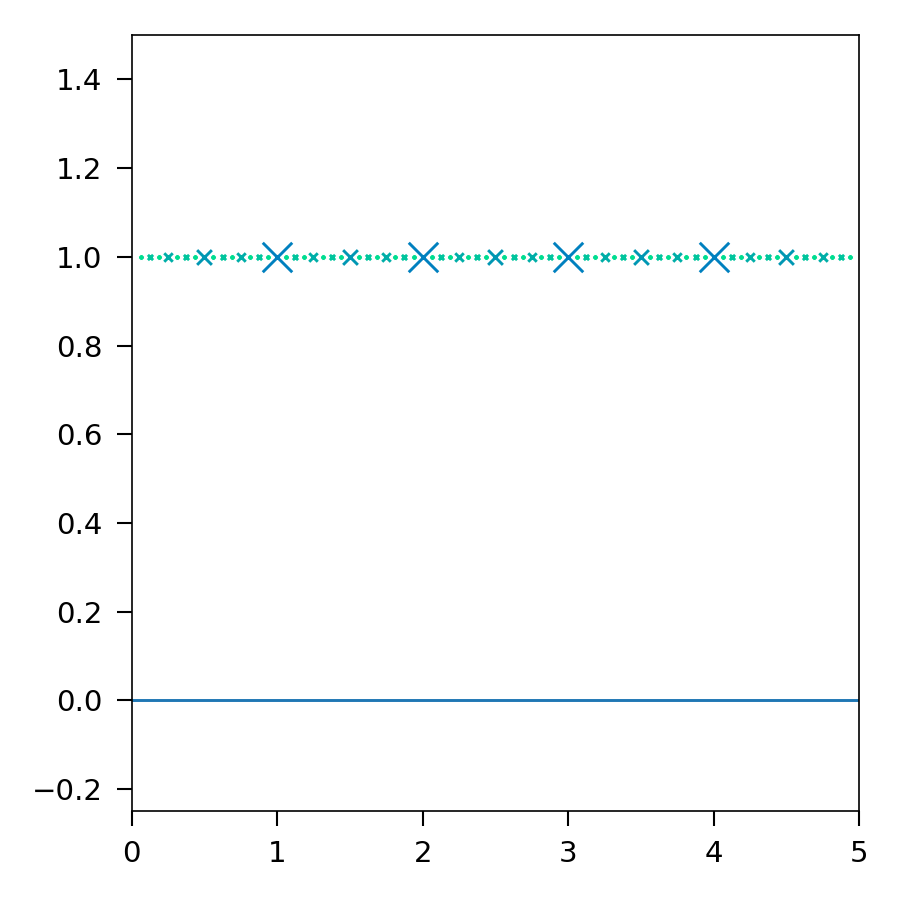
\includegraphics{Code/Rational.png}
	\caption{An illustration of the indicator function $\mathbbm{1}_\Q(x)$, showing a few rationals that are multiples of negative powers of 2.}
	\label{fig:rational}
\end{figure}
\newpage

$\sigma$-algebra \\
A family of subsets of a set. For example, given the set
\begin{equation*}
	\{\hbox{1, 2, 3, 4, 5, 6, 7, 8, 9, 0}\}
\end{equation*}


\end{document}
